\documentclass{article}
\usepackage[utf8]{inputenc}
\usepackage{array}
\usepackage{amsmath, mathtools}
\usepackage{graphicx}
\usepackage{empheq}
\usepackage{float}
\usepackage{listings}
\usepackage{hyperref}
\hypersetup{
    colorlinks=true,
    linkcolor=blue,
    filecolor=magenta,
    urlcolor=cyan,
}

\DeclarePairedDelimiter{\ceil}{\lceil}{\rceil}

\usepackage{color}

%New colors defined below


%Code listing style named "mystyle"
\lstdefinestyle{mystyle}{
  basicstyle=\footnotesize\ttfamily,
  keywordstyle=\bf\ttfamily\color[rgb]{0,.3,.7},
  commentstyle=\color[rgb]{0.133,0.545,0.133},
  stringstyle={\color[rgb]{0.75,0.49,0.07}},
  breaklines=true,
  breakatwhitespace=true,
  breaklines=true,
  captionpos=b,
  keepspaces=true,
  numbers=left,
  numbersep=5pt,
  showspaces=false,
  showstringspaces=false,
  showtabs=false,
  tabsize=2,
  sensitive=true,
}

%"mystyle" code listing set
\lstset{style=mystyle}

% https://tex.stackexchange.com/questions/95838/how-to-write-a-perfect-equation-parameters-description
\newenvironment{conditions}[1][let:]
  {#1 \begin{tabular}[t]{>{$}l<{$} @{${}={}$} l}}
  {\end{tabular}\\[\belowdisplayskip]}


\title{Cassandra Availability with Virtual Nodes}
\author{
  Joseph Lynch\\
  \texttt{joe.e.lynch@gmail.com}
  \and
  Josh Snyder\\
  \texttt{josh@code406.com}
}

\begin{document}

\maketitle

\section{Introduction}
With the addition of \textt{vnodes} \cite{vnodes} in version 1.2, Cassandra
made it easier to balance a dataset across cluster nodes. With vnodes, the
variance of data size held by any one host decreases. vnodes also afford the
ability to easily change the number of hosts participating in a cluster, which
previously was conducive only to doubling and halving.

In return for easier operability, vnodes trade off availability. As we document
in this report, the availability cost of vnodes is quantifiable, and
unavoidable. We present a model of the availability of a single-datacenter
Cassandra cluster under failures. We attempt to predict, for a given cluster
configuration, what availability guarantees are feasible.

Based on our model, we conclude that the Cassandra default of 256 virtual nodes
per physical host is unwise, as it results in steadily rising chance of
unavailability as cluster size grows. This is antithetical to Cassandra's
design goal of fault-tolerance.

\section{Description of the Problem}

Data in Cassandra is distributed across the cluster nodes according to a
hashing algorithm. Data is identified by a partition key. Partition keys are
hashed by a hashing algorithm, yielding a bounded integer. The default
algorithm assigns a 64-bit integer to each partition key. Each node in the
cluster takes responsibility for storing data along a contiguous range of the
integer space.

Cassandra clusters achieve fault-tolerance by storing multiple copies of each
piece of data. The quantity of copies (replication factor) is configurable, but
is typically an odd number, with three being most common. Higher replication
factors achieve greater fault-tolerance, at the cost of increased storage
requirements.

Nodes in a Cassandra cluster are assigned a token: an integer value which fixes
the end of its token range. The start of each range is variable, depending on
the location of tokens held by other nodes in the cluster. To achieve a
replication factor of one, a node's owned token range will extend from its left
neighbor's token to its own. With RF=1, the failure of any node will make that
node's token range unavailable for reads or writes. Since the failure of

So long as any node


In Cassandra's data placement strategy, availability is only compromised if
physical nodes that own the same range fail before nodes can recover. Prior
models attempted to model Cassandra's failure modes \cite{dataloss}, but they
do not take into account the recovery aspect of Cassandra where it
automatically \footnote{Not exactly automatically, but with the right
\href{https://github.com/Netflix/Priam}{automation} it can be automatic}
streams lost data to new replicas. We approach the problem from a different
direction, opting instead to model outages as a combination of losing a single
node plus losing a neighboring node that owns an intersecting token range
before recovery finishes, causing \texttt{UnavailableExceptions} to clients. We
do not care about the proportion of the ring that is unavailable or for how
long as any unavailability is unacceptable to customers. Using this model we
show that the Cassandra default of 256 tokens per node is an unwise choice, and
a drastically smaller default should be chosen to more fairly balance the
tradeoffs.

\section{Analysis}

We conduct our analysis on cluster with RF=3. Before virtual nodes, a Cassandra
node in an RF=3 cluster would inter-depend on exactly 4 other nodes: its two
left-neighbors and its two
right-neighbors.

By siting multiple token ranges within the responsibility of a single server,
virtual nodes increase the interdependency

Virtual nodes decrease availability by coupling physical nodes together, but
they theoretically increase the speed that you can recover nodes \footnote{In
our experience, at least with Cassandra 2.x and 3.0.x, inbound streaming tops
out at significantly under line rate, but this simply makes this model
conservative}. For the purposes of this analysis:

\begin{conditions}
 n       &  number of hosts in the cluster \\
 \lambda &  average failure rate of hosts (1/s) \\
 S       &  size of the dataset per host (MB) \\
 v       &  number of tokens per physical node \\
 R       &  replication factor (number of replicas per token) \\
 B_{inc} &  maximum incoming bandwidth of a joining physical node in (MB/s) \\
 B_{out} &  maximum outgoing bandwidth of a stream (MB/s) \\
\end{conditions}

$n$ and $S$ are details of a particular Cassandra deployment, $v$ and $B_{out}$
are configuration options in \texttt{cassandra.yaml}, $R$ is determined by the
keyspace replication strategy and $\lambda$ and $B_{inc}$ are determined by the
hardware Cassandra is deployed to.

\subsection{Availability Model}

Crucial to the availability calculation is how quickly nodes can recover. The
longer a node takes to recover, the longer a second failure can occur and cause
an outage. We model this with the following equation:

\begin{subequations} \label{recovery}
    \begin{align}
        k & = v * (R - 1) \\ \label{recoverya}
        n_{p} & = n - \frac{n}{R} \\
        E[n_{neighbors}] & = n_{p} * [1 - (1-\frac{1}{n_{p}})^k] \label{recoveryc} \\
        speed & = \min(B_{inc}, E[n_{neighbors}] * B_{out}) \\
        E[T_{recovery}] & = \frac{S}{speed} \\
        E[T_{recovery}] & = \frac{S}{\min(B_{inc}, E[n_{neighbors}] * B_{out})}
    \end{align}
\end{subequations}

Equations \ref{recoverya} through \ref{recoveryc} follow from a slight
simplification of the Cassandra token placement algorithm and the assumption
that the number of racks in a datacenter equals the number of replicas $R$
\cite{replication}. For example, in cloud environments Cassandra racks
generally map 1:1 with availability zones and this assumption holds in every
cloud environment (AWS, GCE, Azure, etc...). Given this assumption, for every
additional token, a physical node gains $R - 1$ replica nodes. This can be seen
as making $v * (R - 1)$ choices of $n - \frac{n}{R}$ distinct items, and asking
what is the expected number of distinct items, which leads to equation
\ref{recoveryc} as this is a variant on the Birthday Problem \cite{neighbors}.
The rest of \ref{recovery} follows from dividing the per node dataset size by
the maximum effective bandwidth to a recovering node. This gives us what we dub
the ``critical window'' where any neighbor failing will cause a token range to
lose quorum.

From equation \ref{recovery} we can see that as $v$ increases, we get faster
streaming until we reach diminishing returns because we have saturated the
inbound network of the joining node. At that point additional streams do not
help speed recovery.

We construct our model for R = 3. Under R = 3, the failure of two
interdependent nodes leaves some token range with only a single active node.
The remaining node can continue to serve reads and writes, but \emph{cannot}
produce a quorum. We consider any lack of quorum, anywhere in the cluster, to
be an outage.

Now that we can model the expected recovery time, we begin the failure model by
assuming that nodes fail as independent Poisson processes with parameter
$\lambda$. Note that modeling node failures as a Poisson process represents a
"best case scenario" for cluster availability: real-life computers are not so
polite that they fail in a manner completely uncorrelated with their peers.

Under such a model the inter-arrival time of node failures follows an
exponential distribution with parameter $\lambda$, and therefore once a single
node failure happens, we lose a second replica of an overlapping range before
the recovery finishes with probability:

\begin{subequations} \label{avail}
\begin{align}
        P(outage|failure) & = F(\tau; \lambda_{eff}) \\ \label{availa}
        P(outage|failure) & = 1 - e^{-\lambda_{eff} * \tau} \\ \label{availb}
        \tau & = E[T_{recovery}] \\ \label{availc}
        \lambda_{eff} & = E[n_{neighbors}] * \lambda \\ \label{availd}
        P(outage|failure) & = 1 - e^{- E[T_{recovery}] * E[n_{neighbors}] * \lambda}
\end{align}
\end{subequations}

Equation \ref{availa} follows from the CDF of an exponential distribution with
parameter $\lambda_{eff}$, and equation \ref{availb} and \ref{availc} follow
because we only care about failures during the recovery period of the
neighboring nodes (which form a combined Poisson process with effective
parameter $\lambda_{eff}$). If we model each node as a splitting Poisson
process with parameter $\lambda$ and splitting probability $P(outage|failure)$,
then each node forms an outage Poisson process with parameter $\lambda_{split}
= \lambda * P(outage|failure)$. If we then join the $n$ such processes, we have
a resulting global Poisson process with parameter $\lambda_{global} =
\lambda_{split} * n$. This yields equation \ref{outage}, which models the
average number of outages over an interval $\tau$.

\begin{empheq}[box=\fbox]{align} \label{outage}
\begin{split}
    E[outages] & = \lambda_{global} * \tau \\
    & = (n * \lambda_{split}) * \tau \\
    & = (n * (\lambda * P(outage|failure))) * \tau \\
    & = (n * (\lambda * (1 - e^{-E[T_{recovery}] * E[n_{neighbors}] * \lambda}))) * \tau
\end{split}
\end{empheq}

From this model we can see that availability is compromised by increasing the
number of nodes ($n$), increasing the failure rate of those nodes ($\lambda$),
increasing the number of tokens per node ($v$), or decreasing the streaming
bandwidth. To see how badly availability reacts with plausible default settings
on a 96 node cluster in a cloud environment with machine failure rate
$\lambda=\frac{0.25}{year}$.

\begin{conditions}
 n       &  96 \\
 \lambda &  $\frac{0.25}{year}$ (7.9e-9 $\frac{1}{s}$) \\
 v       &  256 \\
 R       &  3 \\
 S       &  307,200 (MB, 300 gigabyte) \\
 B_{inc} &  125 (MB/s, 1 gigabit) \\
 B_{out} &  25 (MB/s, 200 megabit) \\
\end{conditions}

Modeling this system for a year, on average we expect ~0.03 failures per year:

\begin{equation}
    \begin{split}
    A & = 96 * 0.25 * (1 - e^{-E[T_{recovery}] * E[n_{neighbors}] * \lambda}) \\
    & = 96 * 0.25 * (1 - e^{-2457 * 64 * 7.927e-9}) \\
    & = 0.029
    \end{split}
\end{equation}

In the case with only \texttt{4} \texttt{vnodes}, the availability is much
better with only ~0.0035 failures per year, a full 10x more availability!

\begin{equation}
    \begin{split}
    A & = 96 * 0.25 * (1 - e^{-E[T_{recovery}] * E[n_{neighbors}] * \lambda} \\
    & = 96 * 0.25 * (1 - e^{-2457 * 7.5 * 7.927e-9}) \\
    & = 0.0035
    \end{split}
\end{equation}


We can clearly see in Fig.\ref{fig:outages_small_vnodes} that small numbers of
vnodes do not appreciably change availability (due to the streaming benefits),
but as the number of vnodes gets large we rapidly lose large amounts of
availability until we level out after the number of vnodes passes the number of
nodes.

\begin{figure}[h!]
    \centering
    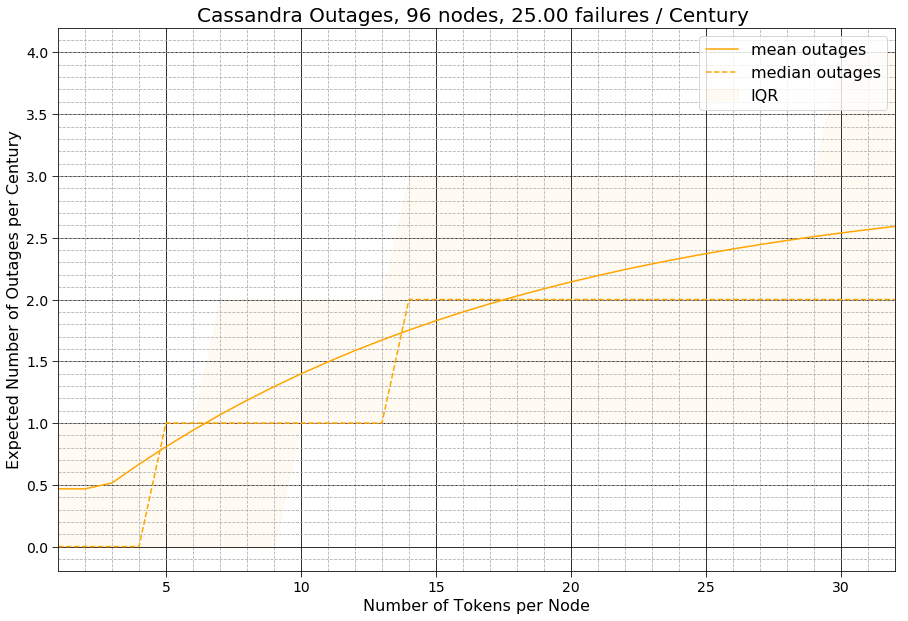
\includegraphics[width=1.0\textwidth]{images/outages_vnodes_small.png}
    \caption{Outages with Small Number of Tokens per Node}
    \label{fig:outages_small_vnodes}
\end{figure}

In Fig.\ref{fig:outages_all_vnodes} we see the effects of varying the failure
rate of machines, and observe that this has a significant impact on the
availability of a Cassandra cluster running with \texttt{vnodes}. In
particular, doubling the rate of machine failures can more than double the
expected number of yearly outages. This makes intuitive sense because as we add
more tokens to each physical node, we are increasing the number of vulnerable
replicas during a single node failure. Rack placement helps a lot to limit the
number of potential replicas to only those residing in other racks, but it is
not enough to prevent likely outage with a high number of tokens per node.

\begin{figure}[h!]
    \centering
    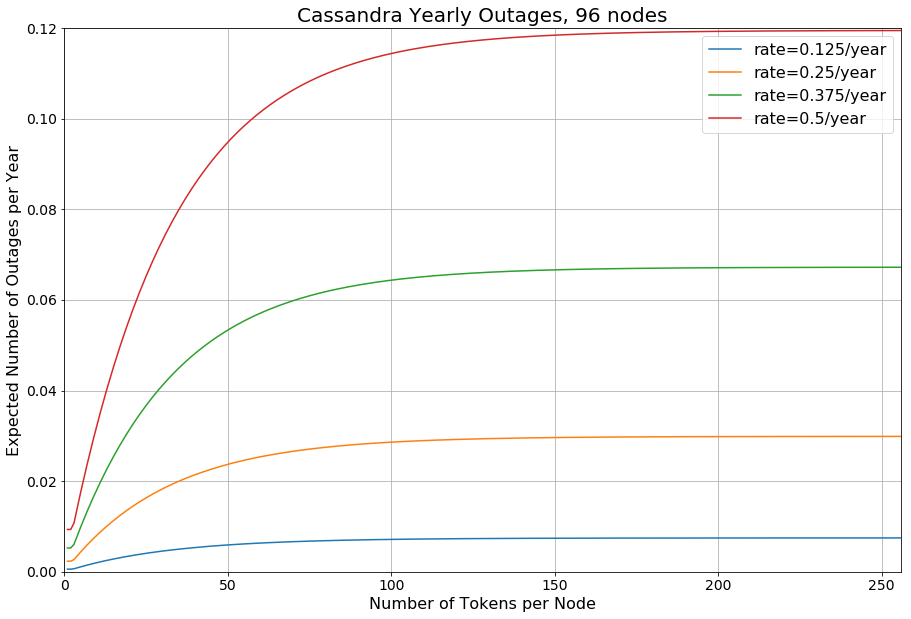
\includegraphics[width=1.0\textwidth]{images/outages_all_vnodes.png}
    \caption{Outages with Varying Tokens per Node}
    \label{fig:outages_all_vnodes}
\end{figure}

It is also interesting to note that as clusters get larger, holding everything
else constant, they become \textit{less available} with more machines. This
intuitively makes sense because as you increase the number of nodes
significantly past RF, you are creating more replicas that can fail and be
vulnerable to a second failure. This is shown in figure Fig.
\ref{fig:outages_nodes}.

\begin{figure}[H]
    \centering
    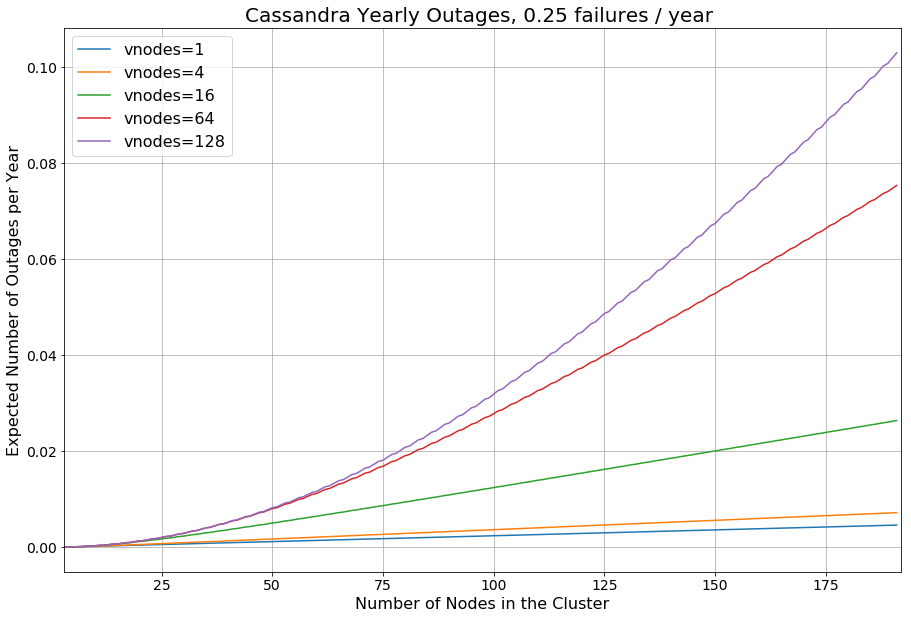
\includegraphics[width=1.0\textwidth]{images/outages_nodes.png}
    \caption{Outages with Varying Nodes in the Cluster}
    \label{fig:outages_nodes}
\end{figure}


\subsection{Virtual Nodes, the Benefits}

Having a number of tokens greater than 1 per physical nodes trades off
availability, but it gains data distribution and operations benefits. In
particular, a major problem pre-$vnode$ was ``hot'' nodes, where one replica
may have significantly more data than other nodes. This was particularly
problematic when scaling up the cluster because in order to keep data evenly
distributed you had to effectively double the cluster. In particular to add
capacity to a cluster of size $n$ with $v$ vnodes you need proportionally fewer
new nodes $N$ to do so. Now that Cassandra token placement is reasonably good
at inserting new tokens where they are needed to balance the ring
\cite{tokenallocation}, we can model the number of nodes needed to scale up
with eq \ref{eq:scaling} as seen in figure \ref{fig:scaling}.

\begin{equation} \label{eq:scaling}
    N = \ceil*{\frac{n}{v}}
\end{equation}

As we can clearly see, as we add more \texttt{vnodes} we must add fewer
physical nodes to the cluster at a time in order to keep it balanced. While 1
token per node requires doubling, 16 tokens per node reduces this, naturally,
by a factor of 16, which is a \textit{significant} improvement. For a 96 node
cluster instead of needing 96 more machines, we can add in increments of 6. The
operational savings only get better as we add more tokens per node, until we
reach the size of the cluster at which point we reach diminishing returns.

\begin{figure}[H]
    \centering
    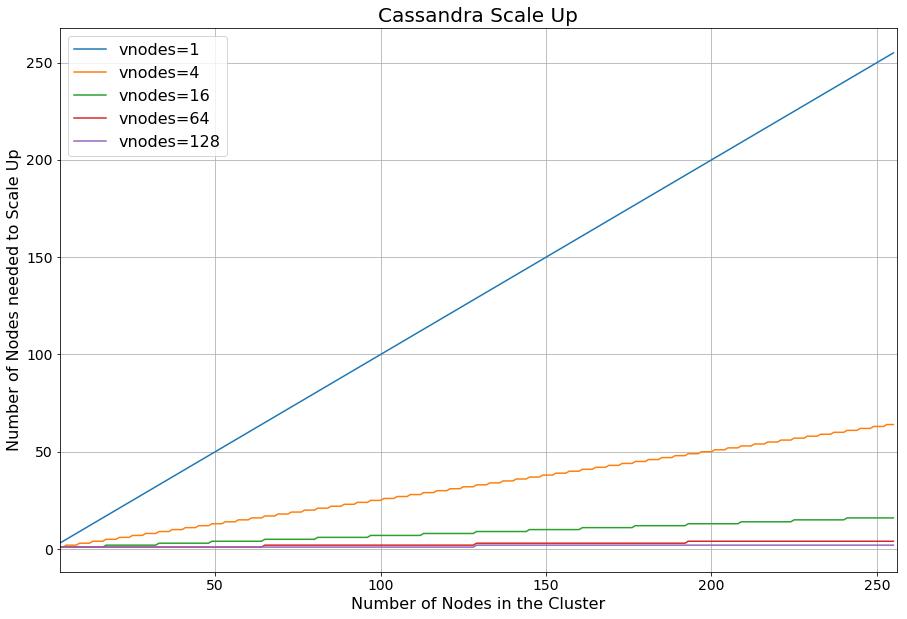
\includegraphics[width=1.0\textwidth]{images/scale_up.png}
    \caption{Nodes Required for Scaling Up}
    \label{fig:scaling}
\end{figure}

\section{Conclusion}

We have shown using a reasonable model that using a number of tokens per node
(\texttt{vnodes}) greater than the number of physical nodes in the cluster
significantly increases the expected outages per year, with default settings
causing up to 10x more outages. This availability is traded away for more even
distribution of data and the ability to add fewer nodes and still maintain even
distribution. We believe, however, that a reasonable middle ground exists in
the \textbf{4-16 vnode range} where the streaming benefits mostly counteract
the additional risky neighbors and therefore the overall probability of outage
is still quite low. At the same time you can still scale up with \textit{10x
fewer} nodes than in the single token case. Changing the default tokens per
node in \texttt{cassandra.yaml} from 256 to 16 would yield \textbf{10x higher
availability} and still have \textbf{10x better scalability} than single token
clusters.

\begin{thebibliography}{9}

\bibitem{vnodes}
Brandon Williams: Virtual nodes in Cassandra 1.2
\\\texttt{https://www.datastax.com/dev/blog/virtual-nodes-in-cassandra-1-2}

\bibitem{karger}
Karger, et. al. Consistent Hashing and Random Trees: Distributed Caching Protocols for Relieving Hot Spots on the World Wide Web
\\\texttt{https://dl.acm.org/citation.cfm?id=258660}

\bibitem{dataloss}
Martin Kleppmann: The probability of data loss in large clusters
\\\texttt{https://martin.kleppmann.com/2017/01/26/data-loss-in-large-clusters.html}

\bibitem{replication}
Cassandra Data replication, \texttt{NetworkAwareTopologyStrategy}
\texttt{https://docs.datastax.com/en/cassandra/latest/cassandra/architecture/archDataDistributeReplication.html}

\bibitem{neighbors}
Kyle Siegrist: The Birthday Problem
\\\texttt{http://www.randomservices.org/random/urn/Birthday.html}

\bibitem{tokenallocation}
Branimir Lambov: New token allocation algorithm in Cassandra 3.0
\\\texttt{https://www.datastax.com/dev/blog/token-allocation-algorithm}



\end{thebibliography}


\section{Appendix}

Source code for all graphs is available on \href{https://github.com/jolynch/python_performance_toolkit/blob/master/notebooks/cassandra_availability/cassandra_availability.ipynb}{github} as well as reproduced below.
\begin{lstlisting}[language=Python]
# coding: utf-8

# In[1]:

from __future__ import print_function
import math
import matplotlib
import numpy as np
import matplotlib.pyplot as plt

get_ipython().magic(u'matplotlib inline')

# Boils down to "If I pick nodes (rf - 1) * vnode times, how many
# distinct nodes will I have in expectation. Note that this is a slightly
# optimistic estimate because Cassandra won't place two replicas of the
# same token on the same machine or rack, but this is close enough for
# the model
# This is a variant of the Birthday Problem where we are insterested
# in the number of distinct values produced
# http://www.randomservices.org/random/urn/Birthday.html
def num_neighbors(n, v, rf):
    k = v * (rf - 1)
    # As cassandra is rack aware, we assume #racks == #replicas
    # This is maybe a bad assumption for some datacenter deployments
    n = n - (n / rf)
    estimate = n * (1.0 - (1.0 - 1.0/n) ** k)
    return max(rf - 1, min(estimate, n))

def p_outage_given_failure(recovery, num_neighbors, rate):
    x =  math.exp(-1 * recovery * num_neighbors * rate)
    return 1 - x

def exp_failures(num_nodes, rate, year):
    return num_nodes * rate * year

def recovery_c(size, bw_in, bw_out, neighbors):
    return int(size / (min(bw_in, neighbors * bw_out)))

nodes = 96
vnodes = 256
rf = 3
# 1000 gigabytes
node_dataset_mb = 300 * 1024
# MB/s
bw_in = 125
bw_out = 25

year = 60.0*60*24*365
arate = 0.25 / year


print("\nFailure Rate Variability")
neighbors = num_neighbors(nodes, vnodes, rf)
print("Neighbors for {0} vnodes: {1}".format(vnodes, neighbors))
recovery = recovery_c(node_dataset_mb, bw_in, bw_out, neighbors)

for i in (0.125, 0.25, 0.5, 1, 2):
    rate = i / (year)
    failures = exp_failures(nodes, rate, year)
    probability = p_outage_given_failure(recovery, neighbors, rate)

    p = "{0:.3f} {1:.2f} {2:.6f} {3:.6f}".format(
        i, failures, probability, failures * probability
    )
    print(p)


def compute_outage(vnodes, failure_rate, num_nodes, rf, bw_in, bw_out):
    neighbors = num_neighbors(num_nodes, vnodes, rf)
    recovery = recovery_c(node_dataset_mb, bw_in, bw_out, neighbors)
    failures = exp_failures(num_nodes, failure_rate, year)
    probability = p_outage_given_failure(recovery, neighbors, failure_rate)
    #p = "{0} {1:.2f} {2:.6f} {3:.6f}".format(
    #    vnodes, neighbors, probability, failures * probability
    #)
    #if vnodes < 32 or vnodes > 255:
    #    print(p)
    return failures * probability


# In[2]:

plt.figure(figsize=(15,10))
plt.title("Cassandra Yearly Outages, {0} nodes".format(nodes, arate * year), fontsize=20)
plt.ylabel("Expected Number of Outages per Year", fontsize=16)
plt.xlabel("Number of Tokens per Node", fontsize=16)
plt.xlim(0, 256)
plt.ylim(0, 0.12)
plt.gca().grid(True)
plt.tick_params(axis='both', which='major', labelsize=14)

num_vnodes = range(1, 257)
rates = [x / year for x in (0.125, 0.250, 0.375, 0.5)]
for rate in rates:
    outages = []
    for vnode in num_vnodes:
        outages.append(compute_outage(vnode, rate, nodes, rf, bw_in, bw_out))
    print(outages[:3])
    plt.plot(num_vnodes, outages, label="rate={0}/year".format(rate*year))
plt.legend(fontsize=16)

outages = [compute_outage(v, arate, nodes, rf, bw_in, bw_out) for v in num_vnodes]
plt.figure(figsize=(15,10))
plt.title(
    "Cassandra Yearly Outages, {0} nodes, {1:.2f} failures / year ".format(
        nodes, arate * year), fontsize=20)
plt.ylabel("Expected Number of Outages per Year", fontsize=16)
plt.xlabel("Number of Tokens per Node", fontsize=16)
plt.xlim(0, 32)
plt.gca().grid(True)
plt.tick_params(axis='both', which='major', labelsize=14)
plt.plot(num_vnodes[:32], outages[:32], color='orange')


# In[3]:

# Hold vnodes constant, vary size of cluster
plt.figure(figsize=(15,10))
plt.title(
    "Cassandra Yearly Outages, {1:.2f} failures / year ".format(
        vnodes, arate * year), fontsize=20)
plt.ylabel("Expected Number of Outages per Year", fontsize=16)
plt.xlabel("Number of Nodes in the Cluster", fontsize=16)
plt.gca().grid(True)
plt.tick_params(axis='both', which='major', labelsize=14)

num_vnodes = (1, 4, 16, 64, 128)
num_nodes = range(3, 192)
for v in num_vnodes:
    outages = [compute_outage(v, arate, n, rf, bw_in, bw_out) for n in num_nodes]
    plt.plot(num_nodes, outages, label="vnodes={0}".format(v))

plt.xlim(3, 192)
plt.legend(fontsize=16)


# In[13]:

# Observe impact of vnodes on Scale Up Balancing
plt.figure(figsize=(15,10))
plt.title("Cassandra Scale Up",fontsize=20)
plt.ylabel("Number of Nodes needed to Scale Up", fontsize=16)
plt.xlabel("Number of Nodes in the Cluster", fontsize=16)
plt.gca().grid(True)
plt.tick_params(axis='both', which='major', labelsize=14)

num_vnodes = (1, 4, 16, 64, 128)
num_nodes = range(3, 256)
for v in num_vnodes:
    scale_up = [math.ceil(float(n) / v) for n in num_nodes]
    plt.plot(num_nodes, scale_up, label="vnodes={0}".format(v))

plt.xlim(3, 256)

plt.legend(fontsize=16)


# In[4]:

import itertools
import random
import sys

def simulate(l):
    return random.expovariate(l)

def offset(values, max_value=sys.maxint):
    nvalues = values[:1] + [0] * (len(values) - 1)
    for i in range(1,len(values)):
        nvalues[i] = values[i] + nvalues[i-1]
    return [n for n in nvalues if n <= max_value]

def outage(o, f_i, t, neighbors):
    failures = 0
    neighbor_indices = range(0, len(o))
    neighbor_indices.remove(f_i)
    random.shuffle(neighbor_indices)
    for n in range(int(round(neighbors))):
        failures += near(o[neighbor_indices[n]], o[f_i], t)
    return failures

def near(a, b, t):
    failures = 0
    for i in a:
        for j in b:
            if j > i + t:
                break
            if j - i > 0 and j - i < t:
                failures += 1
    return failures

def run_simulate(l, neighbors, nodes):
    rs = []
    for r in range(5):
        o = [offset([simulate(l) for j in range(200)]) for i in range(nodes)]
        maxes = [x[-1] for x in o]
        m = max(maxes) / year
        outages_per_year = (sum([outage(o, i, recovery, neighbors) for i in range(nodes)]) / m)
        print("Run {0} gave {1:.3f} outages/year".format(r, outages_per_year))
        rs.append(outages_per_year)
    print("Simulation outages/year: ", sum(rs) / len(rs))

def run_simulate_naive(l, neighbors, nodes):
    p_split = p_outage_given_failure(recovery, neighbors, l)
    l_split = l * p_split
    l_global = nodes * l_split
    rs = []
    for r in range(10):
        events = 10000
        o = offset([simulate(l_global) for j in range(events)])
        ##failure_years = [int(x/year) for x in o]
        num_years = max(o) / year
        rs.append(events / num_years)
    print("Simple simulation outages/year: ", sum(rs) / len(rs))


print(p_outage_given_failure(recovery, num_neighbors(nodes, vnodes, rf), arate))
print(vnodes, arate, nodes, rf, bw_in, bw_out, recovery, num_neighbors(nodes, vnodes, rf))
print("Predicted outages/year:", compute_outage(vnodes, arate, nodes, rf, bw_in, bw_out))
#run_simulate(arate, num_neighbors(nodes, vnodes, rf), nodes)
run_simulate_naive(arate, num_neighbors(nodes, vnodes, rf), nodes)
run_simulate(arate, num_neighbors(nodes, vnodes, rf), nodes)
\end{lstlisting}

\end{document}
